\documentclass{article}

\usepackage{../repsty}
\usepackage{multirow}


\begin{document}
	\title{Analysis of the 2016 data}
	\maketitle
	
\section{Overview}

In the 2016 experiment a polarized proton beam was scattered on a polarized deuterium target. The beam was cooled using electron cooling, and bunched using the COSY RF bunching system. The intensity of the cooling electron beam was 120 mA at injection, and 45 mA during acceleration. Before a cycle, the beam was stacked for 100 seconds (EXP2 $\times$ 5).

The cycles lasted thirteen minutes (792 seconds). In the first half of the cycle the target was turned of, in the second off. The target's spin state remained constant throughout, the beam's alternated through the spin up, down, and null states. In total, there were twelve cycles for each beam spin state. 

The cycles are shown in Figure~\ref{fig:Cycles}; the slopes estimated from those cycles are plotted against time in Figure~\ref{fig:Slopes}; the slopes' summary statistics (only for the target spin state \#1) are aggregated in Table~\ref{tbl:SlpSumStat}.

\begin{figure}
	\centering
	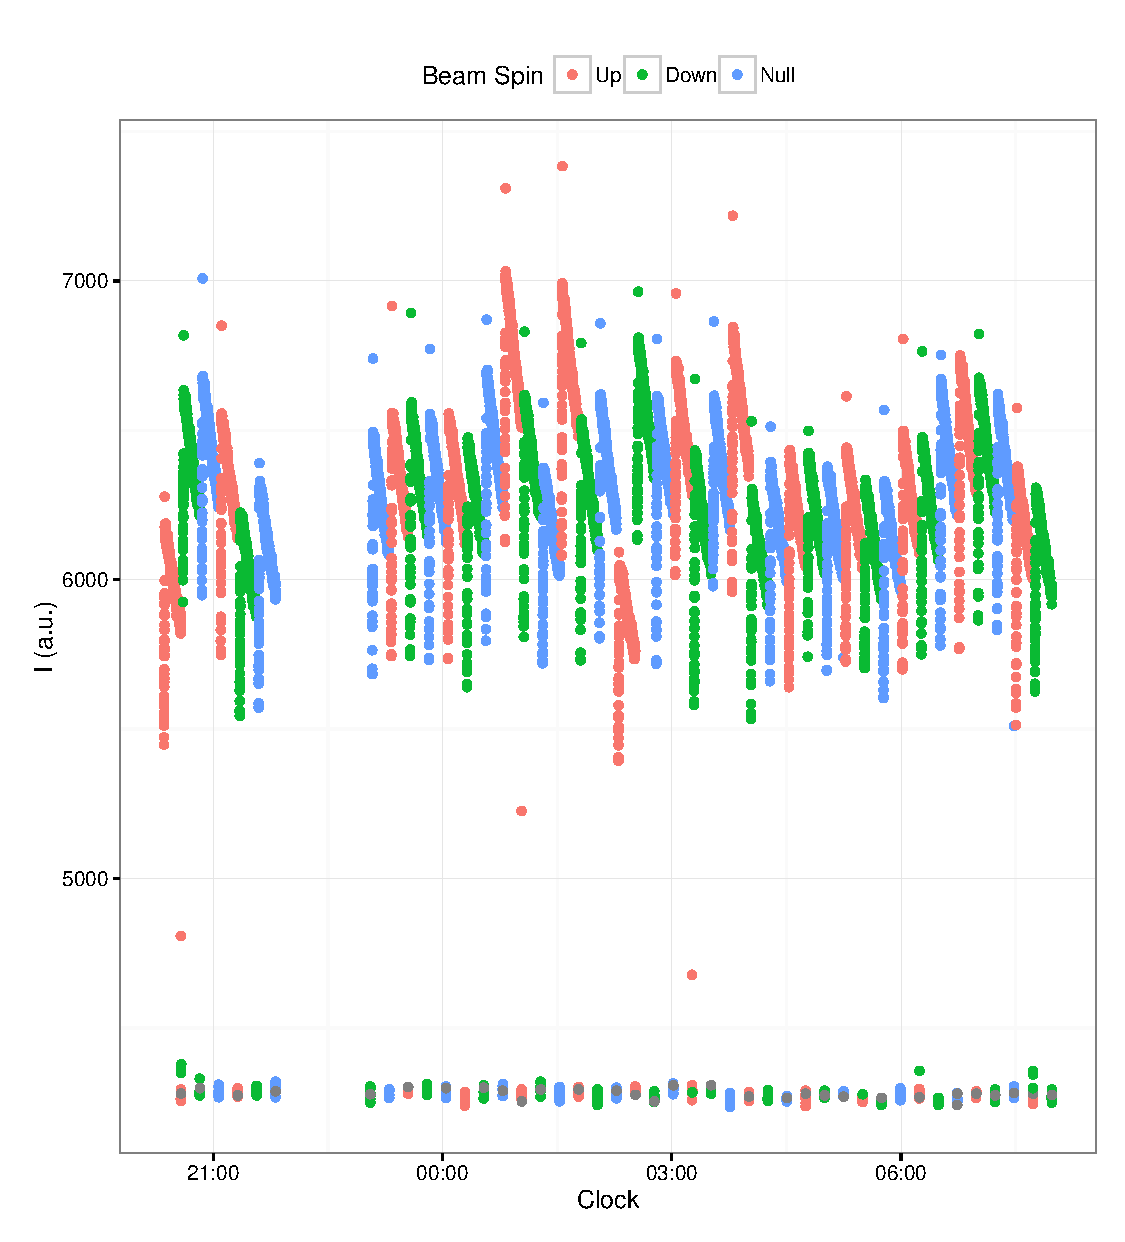
\includegraphics{Cycles2016.eps}
	\caption{Cycles in 2016 colored according to the beam spin state. Before 22:30 the target spin state is 3, after it is 1.\label{fig:Cycles}}
\end{figure}
\begin{figure}
	\centering
	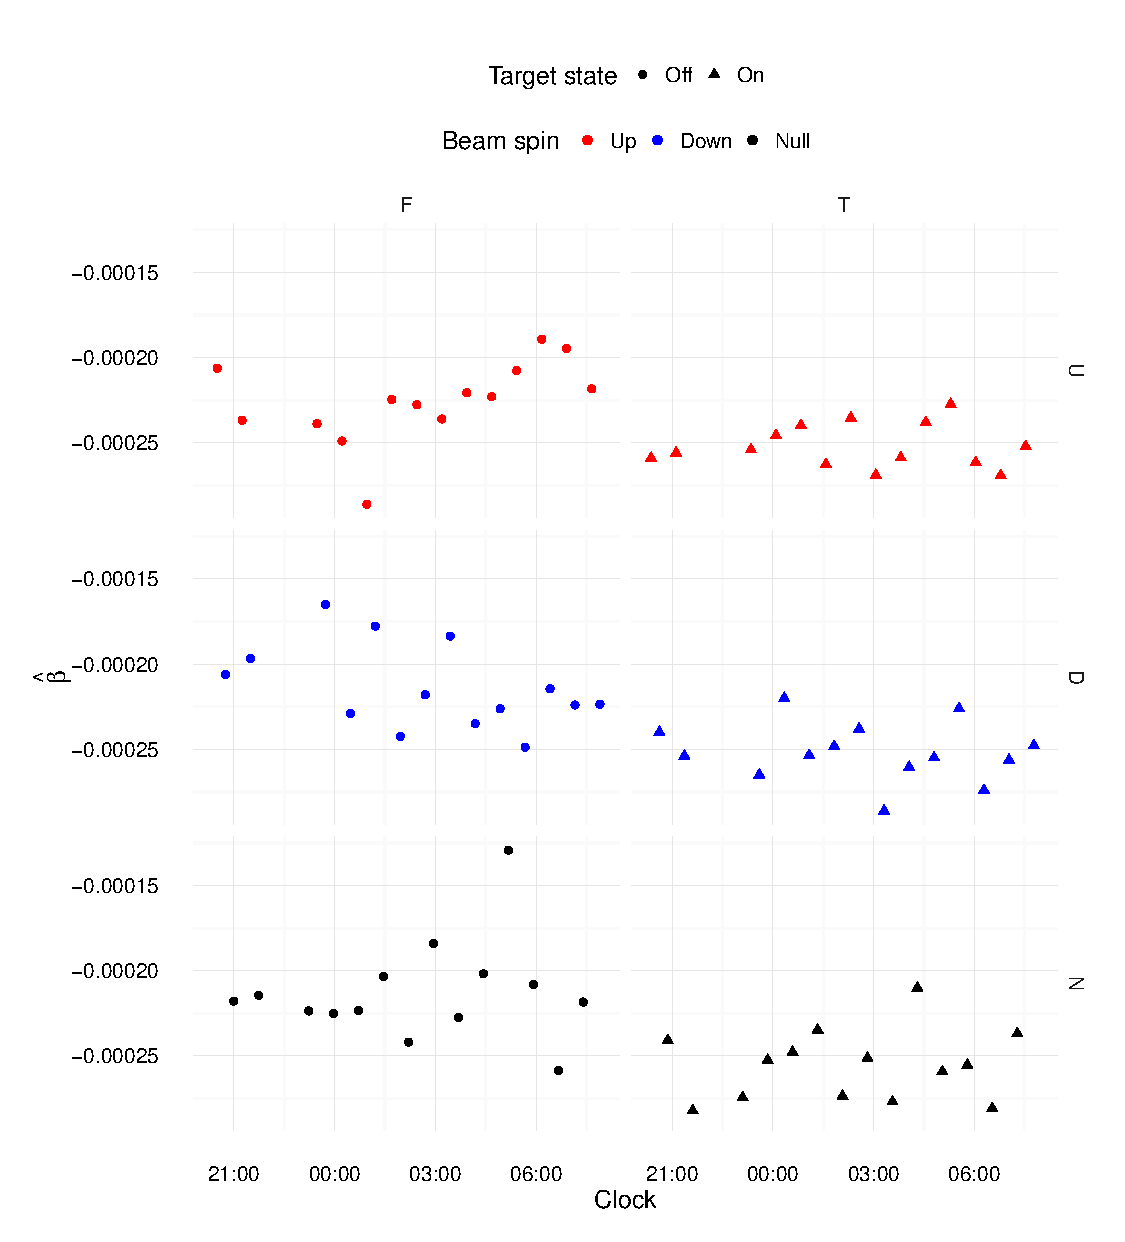
\includegraphics{Slopes2016_VS_Clock.eps}
	\caption{Slope estimates against time.\label{fig:Slopes}}
\end{figure}	
	
\newcommand{\vp}[2]{#1\cdot10^{#2}}
\begin{table}[h]
	\centering
	\caption{Slope summary statistics.\label{tbl:SlpSumStat}}
	\begin{tabular}{lllllrr}
		\hline\hline
		       Target        & Spin & \# & Mean (a.u.)      & SE (a.u.)    \\ \hline
		\multirow{3}{*}{Off} & Up   & 12 & $\vp{-2.26}{-4}$ & $\vp{7}{-6}$ \\
		                     & Down & 12 & $\vp{-2.16}{-4}$ & $\vp{8}{-6}$ \\
		                     & Null & 12 & $\vp{-2.12}{-4}$ & $\vp{9}{-6}$ \\ \hline
		\multirow{3}{*}{On}  & Up   & 12 & $\vp{-2.51}{-4}$ & $\vp{4}{-6}$ \\
		                     & Down & 12 & $\vp{-2.53}{-4}$ & $\vp{5}{-6}$ \\
		                     & Null & 12 & $\vp{-2.54}{-4}$ & $\vp{6}{-6}$ \\ \hline
	\end{tabular}
\end{table}


\section{Properties of the data}
The Gauss-Markov theorem puts certain conditions on the data in order that the least squares slope estimator be minimum variance mean-unbiased. Those conditions are:~\cite{GaussMarkov}
\begin{enumerate}
	\item Linearity and additivity of the relationship;
	\item Independence of the predictor and error variables (strict exogeneity);
	\item No serial correlation of the error;
	\item Constant variance of the error (homoskedasticity).
\end{enumerate}

The Breusch-Pagan test against heteroskedasticity suggests that our data are homoskedastic; however, the Durbin-Watson test for autocorrelation of the residuals (whose statistic is the value of the auto-correlation function at lag 1) yields the statistic around 60\% for all cycles (see Figure~\ref{fig:DW2}). Autocorrelation does not affect the slope estimate itself, but in its presence the OLS estimate of its standard error is biased. To correct for that, we use a robust standard error estimator provided by the \emph{sandwich} package of R.~\cite{RSandwich} The robust estimator takes care of both the (possible) heteroskedasticity, and the autocorrelation. 

\begin{figure}
	\centering
	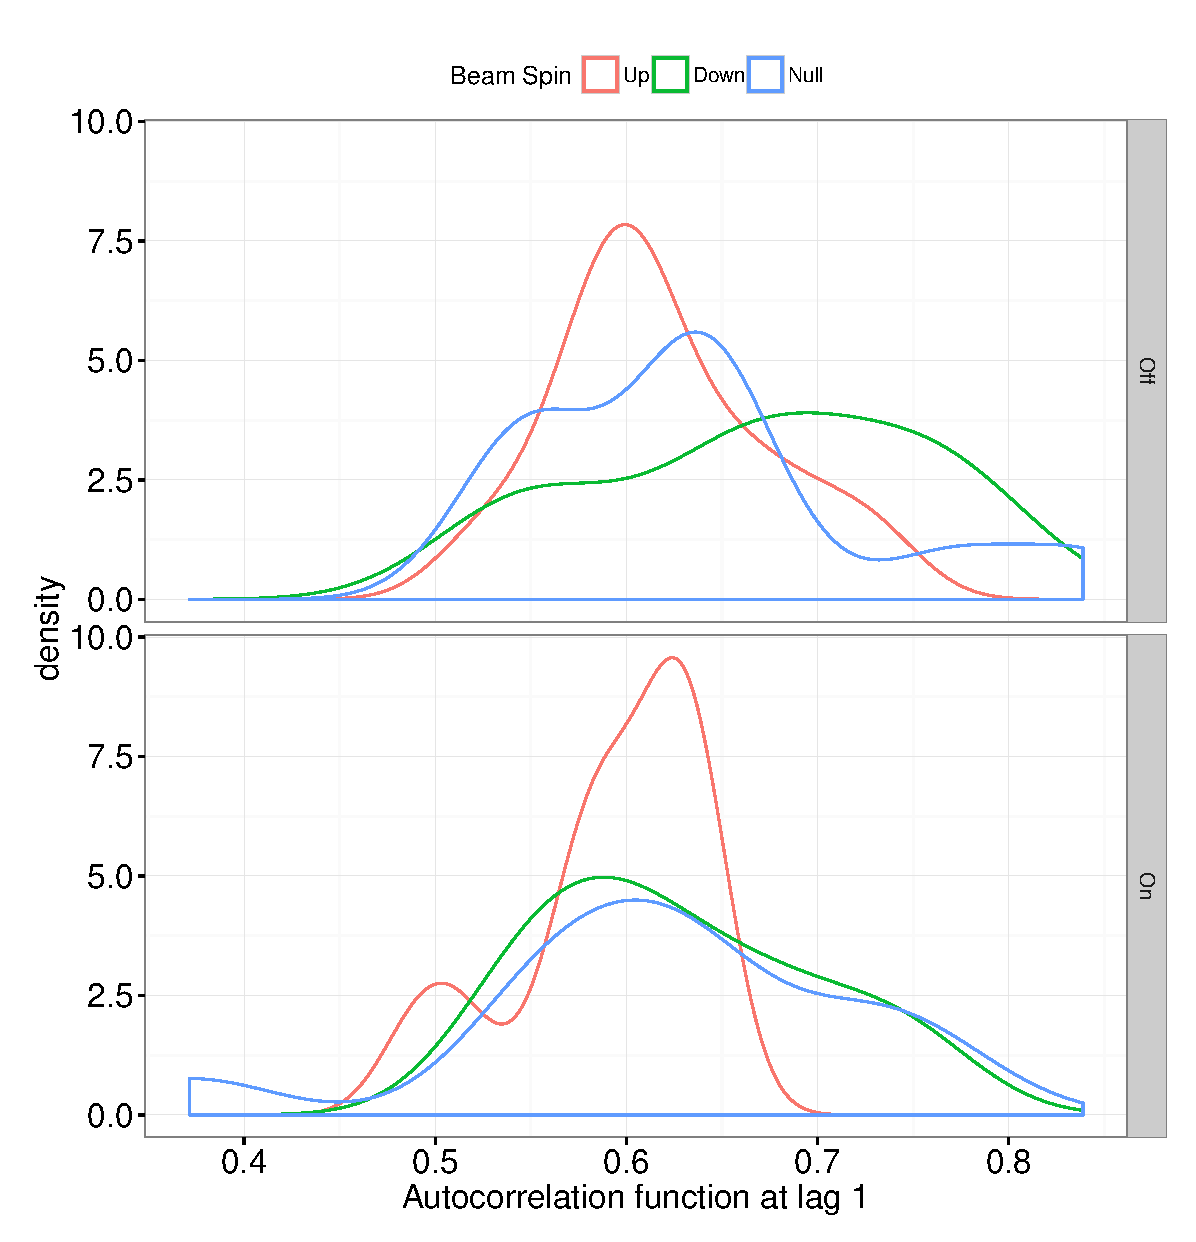
\includegraphics{ACF1_dens.eps}
	\caption{The distribution of the auto-correlation of the residuals at lag 1.\label{fig:DW2}}
\end{figure}

The moving Chow test, as well as other structural tests from the package~\cite{RStrucchange} suggest changes in the slope, i.e. the appropriateness of a piece-wise linear regression. The distribution of the breakpoints, as found by the Chow test, are plotted in Figure~\ref{FStat_BP_dens}.

\begin{figure}
	\centering
	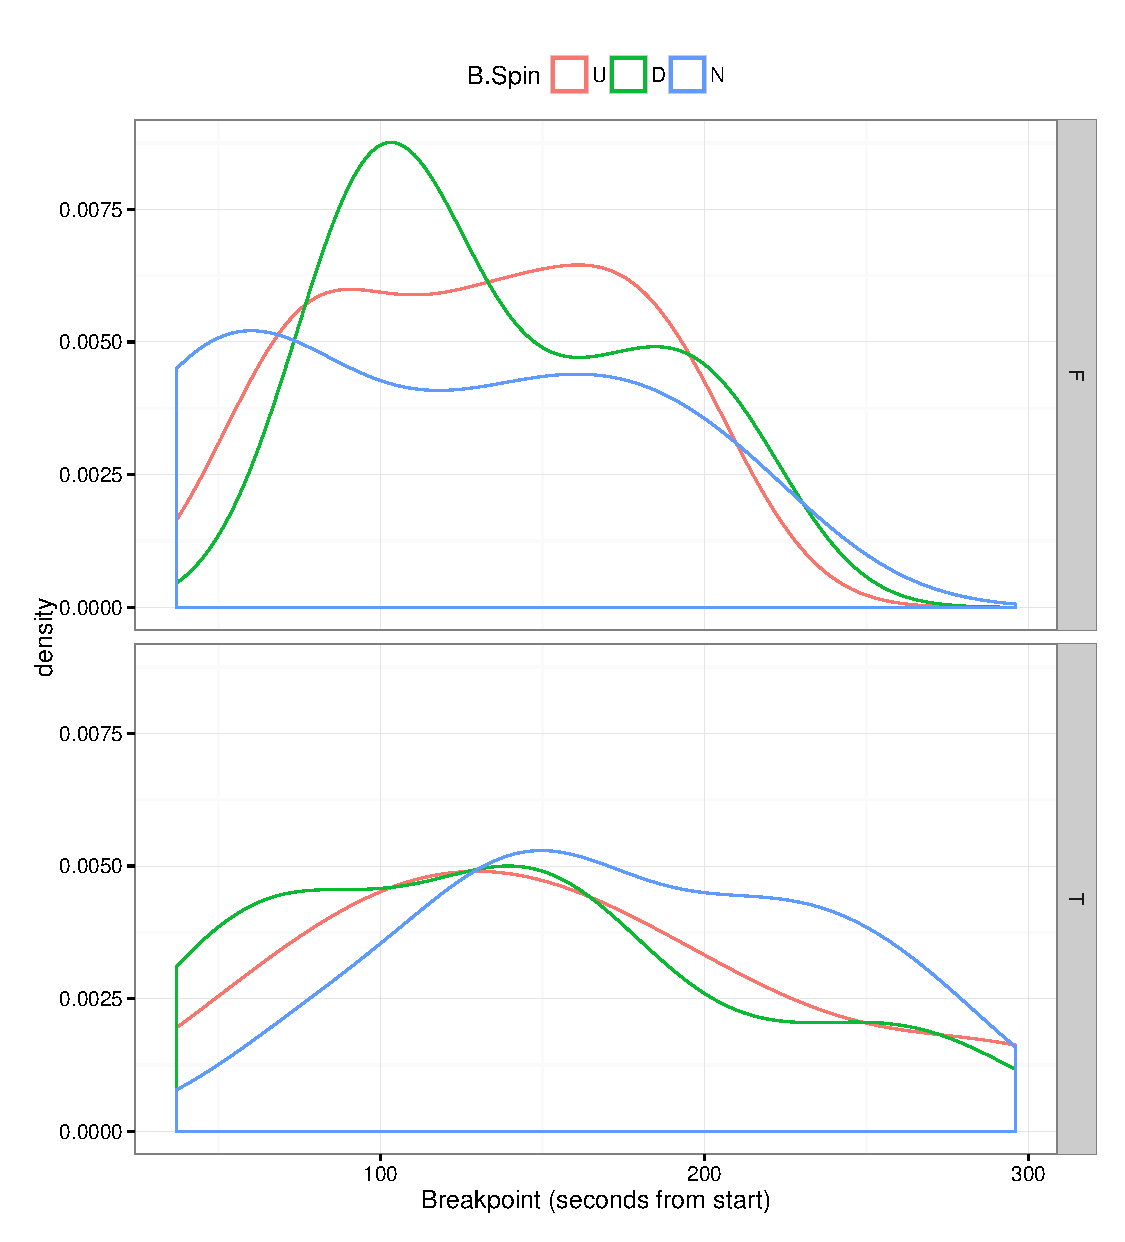
\includegraphics{FStats_BP_dens.eps}
	\caption{Point of change in the slope as found by the moving Chow test. The target-less cycles' distribution is in the upper panel.\label{FStat_BP_dens}}
\end{figure}

\begin{figure}
	\centering
	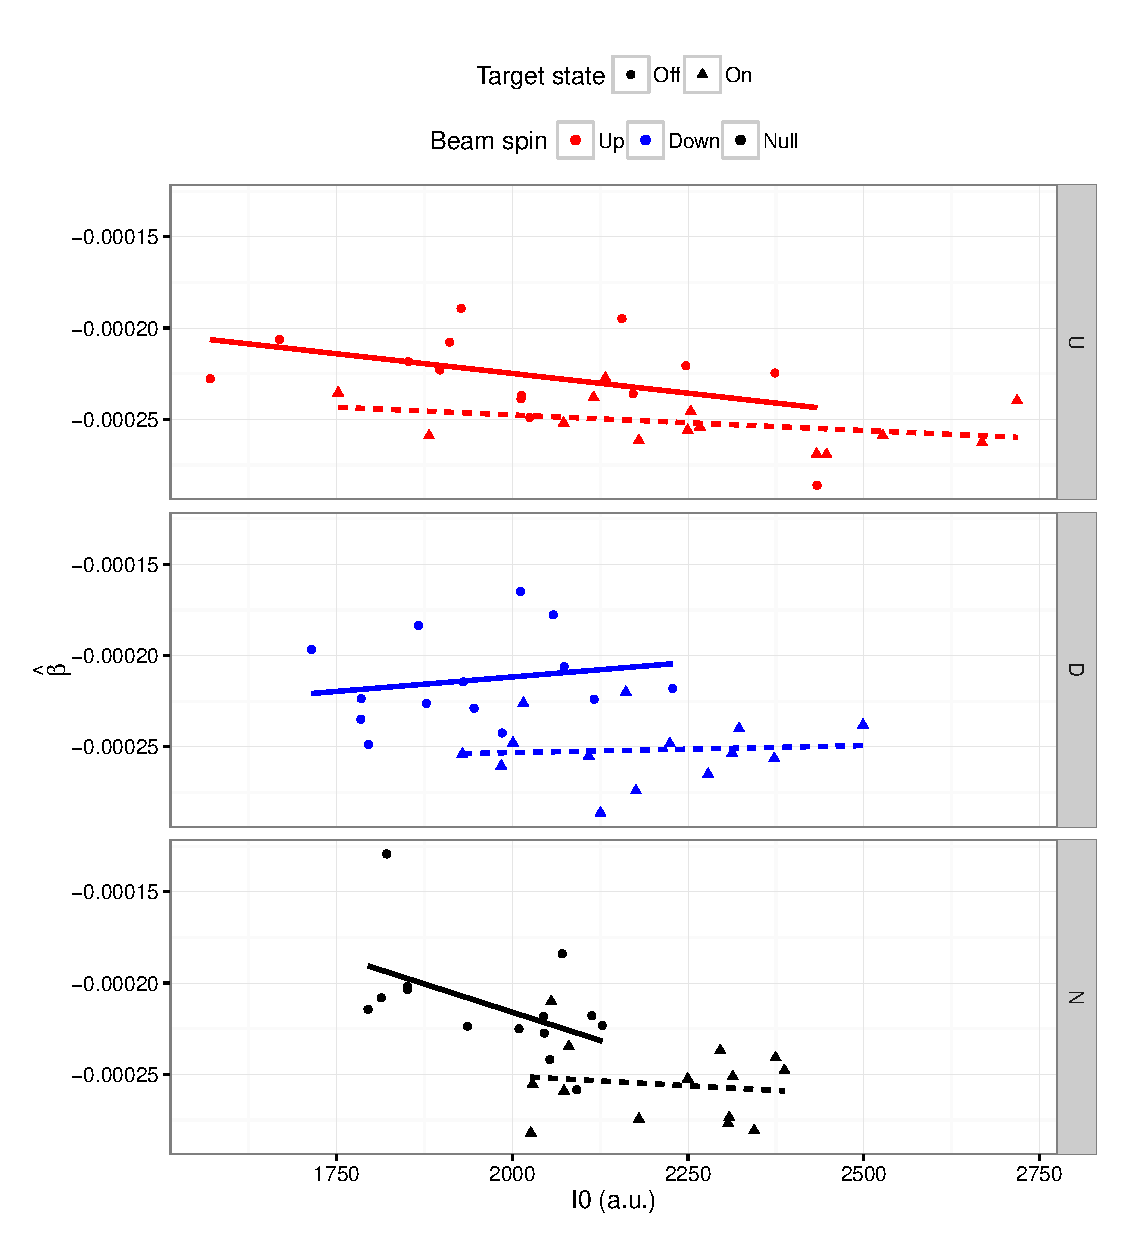
\includegraphics{Slope_VS_IniCurrent_2016.eps}
	\caption{Slope estimates against the initial beam current. The beam current is estimated from the regression model.\label{fig:Slp_VS_I0}}
\end{figure}



\section{Obtainable estimates}

\begin{thebibliography}{9}
	\bibitem{GaussMarkov}
	D.S.G. Pollock. ``Topics in Econometrics.''
	\bibitem{RSandwich}
	\url{https://cran.r-project.org/web/packages/sandwich/sandwich.pdf}
	\bibitem{RStrucchange}
	\url{https://cran.r-project.org/web/packages/strucchange/strucchange.pdf}
\end{thebibliography}

\end{document}